\documentclass[a4paper, twocolumn]{article}
\usepackage[utf8]{inputenc}
\usepackage{amsmath}
\usepackage{graphicx}
\graphicspath{documents/}
\usepackage{caption}
\captionsetup{font=scriptsize}
\usepackage[margin=0.5in]{geometry}

\title{Atomic Spectroscopy}
\author{
Garcia, Jorge A.\\
\and
Lane, Ryan C. \\
\and
Miller, Patrick C.
}
\date{February 14th, 2018\\\line(1,0){500}}

\begin{document}
\maketitle

\section{Purpose}
The purpose of this experiment is to demonstrate the emission lines of the electromagnetic spectrum for different elements.
Diffraction is the key physical concept in this experiment, since an element will emit light it's light as a combination of
its different spectral lines, and it must be diffracted into its components in order to observe them individually. The only
controlled quantity is that of the diffraction grating, while measured quantities during the experiment are that of the 
angles at which emission lines are seen. From these quantities, the wavelength of said emission lines will be determined and
an approximation of the Rydberg constant can be achieved.

\section{Apparatus and Method}
The two essential apparatus for the experiment are the discharge tube and the spectrometer. The discharge tube is lit up with an
electric current with a potential of 5 kV. The bright lamp will be used as the light source for the experiment.

The spectrometer consists of two components: the collimator and the telescope. It is mounted on a base with a pivot that allows
the telescope to move freely in a 180 degree range.

The collimator has a slit at the front end near the discharge tube, which regulates the amount of light entering the spectrometer.
Light then goes through a lens and aligns the incident light to make it into parallel rays. The rays then passes through a
diffraction grating with a predetermined size; the grating used was of 600 lines per mm. The light is then decomposed into its
various individual wavelength components, and the emission lines can be seen by sweeping the telescope along the pivot. As light from
a certain wavelength enters the telescope, a lens converges the incident light into the eyepiece, allowing the user to observe the
emission line.

\section{Procedure}
The procedure was replicated for three different samples. After setting the discharge tube in front of the slit, it is important
to align the telescope to the center of the telescope pivot, so it is perpendicular to the parallel beam. This allows for the 
identification of the central emission line, which will be used as the reference point to find the rest of the lines. The telescope
will then be moved to find a new line, and recording of the angle indicated on the base is necessary. This measured angle has
at the very least an uncertainty of 0.1 degrees from pure instrumental limitations.

The first run was done with Mercury for calibration purposes and ensuring proper use of the equipment, as the tube has a longer
lifetime than that of Hydrogen. Hydrogen will be used to approximate the Rydberg constant. Finally, the spectrum of an unknown source
will be used, with the objective of identifying it.

\section{Data and Uncertainties}
Each member in the team did 2 sets of measurements, one for the left-side lines and another for the right-side. The angle at which
the undiffracted light is seen was not set to 0 degrees, and such all measurements were shifted, so only the change in angle from the center
line is taken into account. The 6 measurements for each of the lines are then averaged, in order to reach a mean value for the angle at which
the color is observed. The standard deviation of the mean is then:
\begin{equation}
 \Delta\theta = \sqrt{\frac{1}{N-1} \sum_{i=1}^{N}(\theta_i-\bar{\theta})^2}
\end{equation}

With N being the number of measurements, $\theta_i$ the ith measurement for an angle, and $\bar{\theta}$ the mean value of that angle.
Calculation of the mean and error of the angles for each emission line was done in Python.

Shown in Table \ref{table:anglesHg} is the average measurements for the Mercury discharge tube. The uncertainty in the mean of each of the angles was
lower than 0.1 degrees, so our uncertainty in these measurements must be instrument dominated. 
\begin{table}[h!]
\centering
\begin{tabular}{ |c||c|c|c| }
 \hline
 \multicolumn{4}{|c|}{\textbf{Mercury (Hg)}} \\
 \hline
 \multicolumn{2}{|c}{\textbf{Degree Shift:}} &
 \multicolumn{2}{|c|}{139.4} \\
 \hline
 \textbf{Color} & $\boldsymbol{\theta}$ & $\boldsymbol{\Delta\theta}$ & \textbf{Order} \\
 \hline
 Violet & 15.1 & 0.1 & First \\
 \hline
 Green & 19.2 & 0.1 & First\\ 
 \hline
 Yellow & 20.3 & 0.1 & First \\
 \hline
 Orange & 20.4 & 0.1 & First \\
 \hline
\end{tabular}
\caption{Average Measurements for Hg}
\label{table:anglesHg}
\end{table}

For the measurements of Hydrogen emission lines (Table \ref{table:anglesH}), the human error was larger than for the 
previous measurements. This is possibly due to the lower intensity of the emission lines, making them harder to be seen.
\begin{table}[h!]
\centering
\begin{tabular}{ |c||c|c|c| }
 \hline
 \multicolumn{4}{|c|}{\textbf{Hydrogen (H)}} \\
 \hline
 \multicolumn{2}{|c}{\textbf{Degree Shift:}} &
 \multicolumn{2}{|c|}{139.4} \\
 \hline
 \textbf{Color} & $\boldsymbol{\theta}$ & $\boldsymbol{\Delta\theta}$ & \textbf{Order} \\
 \hline
 Violet & 15.1 & 0.1 & First \\
 \hline
 Cyan & 17.0 & 0.2 & First \\ 
 \hline
 Red & 23.3 & 0.2 & First \\
 \hline
 Blue & 35.75 & 0.3 & Second \\
 \hline
\end{tabular}
\caption{Average Measurements for H}
\label{table:anglesH}
\end{table}
\vfill\eject
The most problems occurred with the Unknown Sample A (Table \ref{table:anglesA}). The emission lines were too faint to be accurately measured, even after
attempts of darkening the room. Because of these difficulties and lack of time to take more measurements, our data is very
imprecise. This especially can be seen in the last two angles.
\begin{table}[h!]
\centering
\begin{tabular}{ |c||c|c|c| }
 \hline
 \multicolumn{4}{|c|}{\textbf{Unknown Sample A}} \\
 \hline
 \multicolumn{2}{|c}{\textbf{Degree Shift:}} &
 \multicolumn{2}{|c|}{139.4} \\
 \hline
 \textbf{Color} & $\boldsymbol{\theta}$ & $\boldsymbol{\Delta\theta}$ & \textbf{Order} \\
 \hline
 1 & 14.4 & 0.2 & First \\
 \hline
 2 & 14.4 & 0.3 & First \\
 \hline
 3 & 15.5 & 0.1 & First \\
 \hline
 4 & 17.7 & 2.1 & First \\
 \hline
 5 & 23.2 & 5.3 & First \\
 \hline
\end{tabular}
\caption{Average Measurements for Unknown Sample A}
\label{table:anglesA}
\end{table}

The separation between the lines of the diffraction grating (slit size), is:
\begin{equation*}
 d = \frac{1}{600 \frac{lines}{mm}} = 1.\bar{6} \mu m
\end{equation*}

And given its precision of 0.01\%, as stated in the lab writeup, its uncertainty would then be:
\begin{equation*}
 \Delta d = 0.1\bar{6} nm
\end{equation*}
So the uncertainty in the incident light is mostly due to the glass from the discharge tube, as this error from the diffraction grating is
immensely small.

\section{Analysis and Uncertainties}
\subsection{Mercury}
Knowing the angle at which an emission line is seen, and given the spacing of the diffraction grating lines, the
wavelengths can be calculated as:
\begin{equation*}
 dsin\theta = m\lambda
\end{equation*}
\begin{equation}
 \lambda = \frac{dsin\theta}{m}
\end{equation}
Accordingly, when calculating the wavelength, the error from the angle of the emission line propagates as follows:
\begin{equation}
 \Delta\lambda = \frac{1}{m} \sqrt{ sin^2\theta (\Delta d)^2 + d^2 cos^2\theta (\Delta\theta)^2 }
\end{equation}

The results were then calculated in Python using Equations 2 and 3.

For Mercury, the found wavelengths are shown in Table \ref{table:lambdaHg}. By plotting the found wavelength against
the sine of the measured angle for each emission line (radians), one should be able to fit a linear function with a slope
equal to that of the spacing between lines in the diffraction grating, since:
\begin{align*}
 dsin\theta &= m\lambda \\
 d &= \frac{m\lambda}{sin\theta}
\end{align*}

With the uncertainty for $sin\theta$ being:
\begin{equation*}
 \Delta sin\theta = (\Delta\theta) cos\theta
\end{equation*}

Using a Linear Least Squares fit, the plot of the model and the data can be seen in Figure \ref{fig:mercury}.
\begin{table}[h!]
\centering
\begin{tabular}{ |c||c|c| }
 \hline
 \multicolumn{3}{|c|}{\textbf{Mercury (Hg)}} \\
 \hline
 \textbf{Color} & $\boldsymbol{\lambda}$ $(nm)$ & $\boldsymbol{\Delta\lambda}$ $(nm)$ \\
 \hline
 Violet & 434.6 & 2.8 \\
 \hline
 Green & 548.6 & 2.7 \\ 
 \hline
 Yellow & 577.8 & 2.7 \\
 \hline
 Orange & 581.4 & 2.7 \\
 \hline
\end{tabular}
\caption{Determined wavelengths and $sin\theta$ for Hg}
\label{table:lambdaHg}
\end{table}

\begin{figure}[h!]
 \centering
 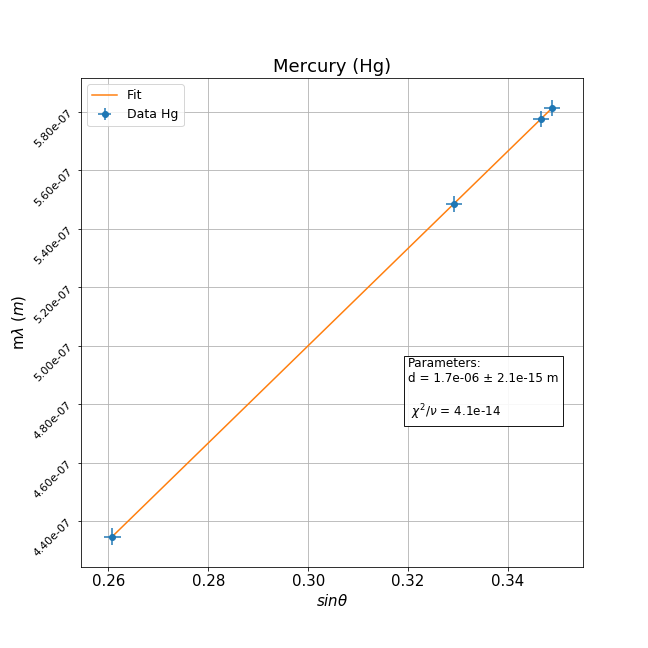
\includegraphics[scale = 0.4]{mercury}
 \caption{Plot of Mercury's $sin\theta$ against $m\lambda$}
 \label{fig:mercury}
\end{figure}

The calculated value for the spacing size d is as expected (equal to its nominal value), and well within the uncertainties of the actual spacing.

\subsection{Hydrogen}
The expected observed wavelengths from the Hydrogen discharge tube can be calculated with the Rydberg formula (Equation 4, Rydberg constant $R = 10 973 731.6$ $m^{-1}$). 
After calculating the possible emission combinations of $n_i$ and $n_f$ spanning from 1 through 10, the only lines in the visible spectrum are the known Balmer series lines
(Table \ref{table:balmer}).
\begin{equation}
 \frac{1}{\lambda} = R(\frac{1}{n_f^2} - \frac{1}{n_i^2})
\end{equation}

With our determined wavelengths of the observed emission lines in Hydrogen (Table \ref{table:lambdaH}, a comparison is made between the observed and the expected
wavelengths (Table \ref{table:comparisonH}).
\begin{table}[h!]
\centering
\begin{tabular}{ |c|c|c|c|c|c| }
 \hline
 \multicolumn{5}{|c|}{\textbf{Hydrogen Balmer Series}} \\
 \hline
 \multicolumn{1}{|c|}{} & \multicolumn{4}{|c|}{$\boldsymbol{n_i}$} \\
 \hline
 $\boldsymbol{n_f}$ & 3 & 4 & 5 & 6 \\
 \hline
 2 & 656.1 nm & 486.0 nm & 433.9 nm & 410.0 nm \\
 \hline
\end{tabular}
\caption{Expected wavelengths for electron transitions of H}
\label{table:balmer}
\end{table}

\begin{table}[h!]
\centering
\begin{tabular}{ |c|c|c| }
 \hline
 \multicolumn{3}{|c|}{\textbf{Hydrogen (H)}} \\
 \hline
 \textbf{Color} & $\boldsymbol{\lambda}$ $(nm)$ & $\boldsymbol{\Delta\lambda}$ $(nm)$ \\
 \hline
 Violet & 435.1 & 3.5 \\
 \hline
 Blue & 486.8 & 3.1 \\
 \hline
 Cyan & 487.3 & 4.8 \\ 
 \hline
 Red & 657.9 & 4.0 \\
 \hline
\end{tabular}
\caption{Determined wavelengths for H}
\label{table:lambdaH}
\end{table}

The wavelength of 410 nm was missing from the measurements, and this might be due to it being near the lower limit of the visible range and thus making it
hard to detect. There is also the repeated lines that, within their uncertainties, include the 486 nm wavelength.
\begin{table}[h!]
\centering
\begin{tabular}{ |c|c|c|c|c| }
 \hline
 \multicolumn{5}{|c|}{\textbf{Hydrogen (H)}} \\
 \hline
 $\boldsymbol{n_i}$ & $\boldsymbol{n_f}$ & $\boldsymbol{\lambda_{th}}$  $(nm)$ & $\boldsymbol{\lambda_{exp}}$  $(nm)$ & $\boldsymbol{\Delta\lambda_{exp}}$ $(nm)$ \\
 \hline
 3 & 2 & 656.1 & 657.9 & 4.0 \\
 \hline
 4 & 2 & 486.0 & 486.8 & 3.1 \\
 \hline
 5 & 2 & 433.9 & 435.1 & 3.5 \\ 
 \hline
 6 & 2 & 410.0 & & \\
 \hline
\end{tabular}
\caption{Comparison of theoretical and experimental wavelengths for H}
\label{table:comparisonH}
\end{table}

An approximation for the Rydberg constant can then be reached by looking at the slope of a function that fits the plot $\frac{1}{n_i^2}$ against $\frac{1}{\lambda}$.
This is shown in Figure \ref{fig:hydrogen}.
\begin{figure}[h!]
 \centering
 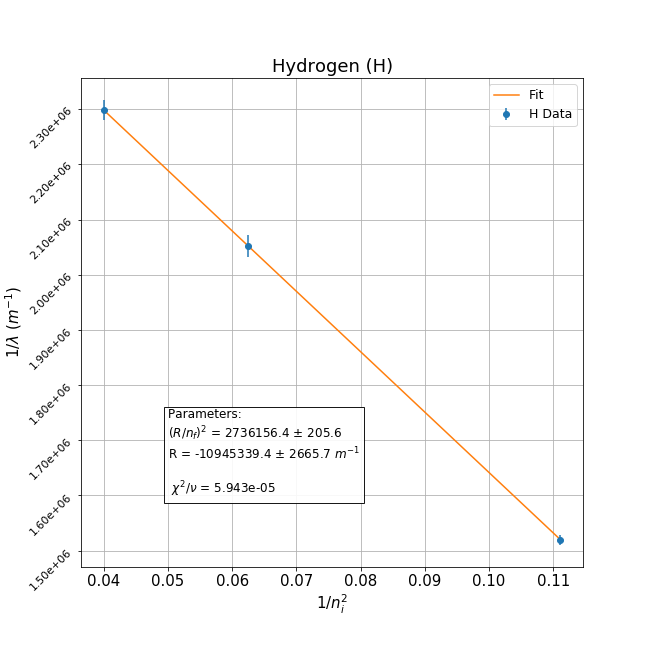
\includegraphics[scale = 0.4]{hydrogen}
 \caption{Plot of Hydrogen's $\frac{1}{n^2_i}$ against $\frac{1}{\lambda}$}
 \label{fig:hydrogen}
\end{figure}

The experimental value of the Rydberg constant is close to its nominal value, although not within the approximation's uncertainties. This is most likely due to the
issues had when attempting to identify the angle at which the various emission lines can be seen for the Hydrogen discharge tube.
\begin{equation*}
\left|\frac{R_{exp}-R_{th}}{R_{th}}\right| = 0.3\%
\end{equation*}

\subsection{Unknown Sample A}

The wavelengths of the seen emission lines were calculated from what few angles obtained. This resulted in imprecise measurements as can be seen in Table \ref{table:lambdaA}:
\begin{table}[h!]
\centering
\begin{tabular}{ |c||c|c| }
 \hline
 \multicolumn{3}{|c|}{\textbf{Unknown Sample A}} \\
 \hline
 \textbf{Color} & $\boldsymbol{\lambda}$ $(nm)$ & $\boldsymbol{\Delta\lambda}$ $(nm)$ \\
 \hline
 1 & 415.9 & 4.2 \\
 \hline
 2 & 415.9 & 7.0 \\
 \hline
 3 & 445.4 & 3.2 \\
 \hline
 4 & 506.7 & 5.8 \\
 \hline
 5 & 655.2 & 1.2 \\
 \hline
\end{tabular}
\caption{Determined wavelengths for Unknown Sample A}
\label{table:lambdaA}
\end{table}

After comparing to the provided emission wavelengths in the lab writeup, these wavelengths are mostly comparable to those of Argon within 2$\sigma$, 
with both values being compared in Table \ref{table:comparisonA}.

\begin{table}[h!]
\centering
\begin{tabular}{ |c|c|c| }
 \hline
 \multicolumn{3}{|c|}{\textbf{Unknown Sample A}} \\
 \hline
 $\boldsymbol{\lambda_{nom}}$ $(nm)$ & $\boldsymbol{\lambda_{exp}}$ $(nm)$ & $\boldsymbol{\Delta\lambda_{exp}}$  $(nm)$ \\
 \hline
 415.9 & 415.9 & 4.2 \\
 \hline
 416.4 & 415.9 & 7.0 \\
 \hline
 451.0 & 445.4 & 3.2 \\ 
 \hline
 518.8 & 506.7 & 5.8 \\
 \hline
 641.6 & 655.2 & 1.2 \\
 \hline
\end{tabular}
\caption{Comparison of nominal wavelengths for Ar and experimental wavelengths for Sample A}
\label{table:comparisonA}
\end{table}

\section{Results}
The best results were obtained from the calibration run with Mercury, being able to accurately and precisely determine the value for the slit size of the diffraction grating.
Problems arose when attempting to observe elements whose emission lines were fainter, those of Hydrogen and Argon, resulting in imprecise data and inaccurate results.
The measured Rydberg constant was off by 0.3\% from its actual value, and a precise fit was achieved. Uncertain results where seen with the
Unknown Sample A, with the calculated wavelengths not being well descriptive of the exact element in the discharge tube, and the closest match is that of Argon.

\section{Conclusions}
We were able to complete the objectives of this experiment. The calculated slit size was precise, and the Rydberg constant was somewhat accurate,
but determining the unknown sample was inaccurate due to uncertainties propagating from our measurements. 
This gives insight into taking further care in measurements in future experiments.

\end{document}